\documentclass[border=4pt]{standalone}
\usepackage[T1]{fontenc}
\usepackage{mathpazo}
\usepackage{tikz}
\definecolor{DarkRed}{rgb}{0.7,0,0}

\begin{document}
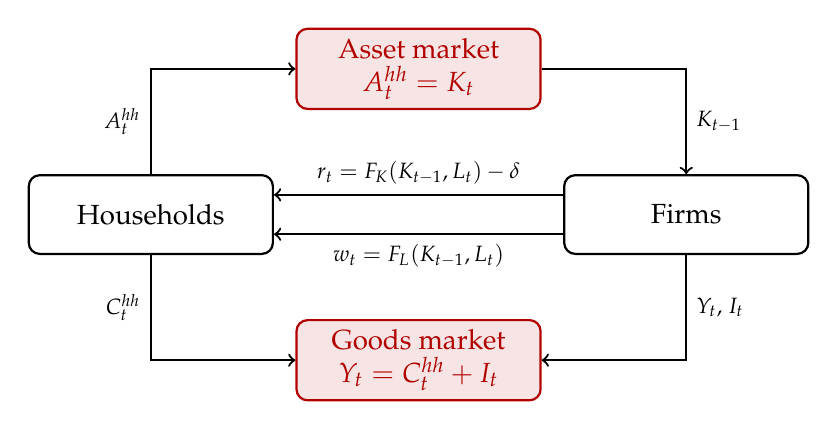
\begin{tikzpicture}[
block/.style={draw,thick,rounded corners,minimum width=3.1cm,minimum height=1cm,align=center},
mkt/.style={block,draw=DarkRed,text=DarkRed,fill=DarkRed!10},
lbl/.style={font=\footnotesize}]

\node[block] (hh) at (0,0) {Households};
\node[block] (firm) at (6.8,0) {Firms};
\node[mkt] (asset) at (3.4,1.85) {Asset market\\$A_{t}^{hh}=K_{t}$};
\node[mkt] (goods) at (3.4,-1.85) {Goods market\\$Y_{t}=C_{t}^{hh}+I_{t}$};

\draw[->,thick] ([yshift=2.5mm]firm.west) -- node[lbl,above]{$r_{t}=F_{K}(K_{t-1},L_{t})-\delta$} ([yshift=2.5mm]hh.east);
\draw[->,thick] ([yshift=-2.5mm]firm.west) -- node[lbl,below]{$w_{t}=F_{L}(K_{t-1},L_{t})$} ([yshift=-2.5mm]hh.east);
\draw[->,thick] (hh.north) |- node[lbl,pos=0.25,left]{$A_{t}^{hh}$} (asset.west);
\draw[->,thick] (hh.south) |- node[lbl,pos=0.25,left]{$C_{t}^{hh}$} (goods.west);
\draw[->,thick] (asset.east) -| node[lbl,pos=0.75,right]{$K_{t-1}$} (firm.north);
\draw[->,thick] (firm.south) |- node[lbl,pos=0.25,right]{$Y_{t}$, $I_{t}$} (goods.east);

\end{tikzpicture}
\end{document}
